\addtocontents{xms}{\protect\addvspace{10pt}}
\chapter{El Llenguatge de Programació Python}\label{chap:python-llenguatge}\index{Python}

\lstset{
	language=Python,
	numbers=none,
	frame=none,
	morekeywords=[1]{as,None,match,case,with}
}

\section{Introducció}

El llenguatge de programació Python va néixer de la mà del programador neerlandès Guido van Rossum l'any 1991 amb la versió 0.9.0, i des de llavors  ha evolucionat de forma continuada: la versió 1.0.0 apareixia l'any 1994, la versió 2.0.0 l'any 2000, i la versió 3.0.0 l'any 2008. La versió 3 va portar grans canvis al llenguatge, de tal manera que va deixar de ser totalment compatible amb la versió 2. Les dues branques del llenguatge --- Python 2 i Python 3 --- van seguir desenvolupant-se en paraŀlel fins a l'any 2020, amb l'última versió  2.7.18  de la branca Python 2. La branca Python 3 segueix desenvolupant-se de forma activa.

Tots els programes d'aquest llibre estan escrits en Python 3, i s'han executat amb la versió 3.10.5.

Python és un llenguatge de codi obert, això vol dir que és accessible per a tothom de forma gratuïta i que es pot distribuir sense restriccions.  Avui  dia el llenguatge Python el desenvolupa i manté la \textit{Python Software Foundation} (PSF); el seu web (\href{https://www.python.org/}{www.python.org}) és el primer lloc a tenir en compte per obtenir el llenguatge i per trobar-ne informació. Hi ha versions disponibles per a molts sistemes operatius: Windows, Linux/UNIX, HP-UX, MacOS, Android, iOS, VMS, Solaris, etc.

Python guanya adeptes cada any, essent un dels llenguatges amb un creixement més fort d'usuaris. Els principals camps d'aplicació on s'està utilitzant aquest llenguatge avui dia són:
\begin{itemize}
	\item Desenvolupament Web.
	\item Jocs.
	\item Aplicacions científiques i numèriques.
	\item Inteŀligència artificial i aprenentatge automàtic --- \textit{machine learning}, en anglès.
	\item Desenvolupament de software.
	\item Processament d'imatges i disseny gràfic.
	\item Anàlisis i visualització de dades.
\end{itemize}

La popularitat d'aquest llenguatge es deu en part al fet que incorpora de sèrie una colla de llibreries que donen accés directe, sense necessitat de programació, a funcions d'àmbit molt diferent, com ara:
\begin{itemize}
	\item  Matemàtiques amb valors reals i complexos, valor reals amb precisió definida, fraccions, generació de nombres aleatoris.
	\item Manipulació de text Unicode i cerca amb expressions regulars.
	\item Càlculs amb dates, hores i calendaris.
	\item Accés a funcions del sistema operatiu.
	\item Compressió de dades: ZIP, GZIP, LMA, etc.
	\item Serveis criptogràfics.
	\item Xarxes i comunicacions.
	\item Manipulació de fitxers HTML i XML.
	\item Protocols d'Internet: URL, HTTP, FTP, etc.
	\item Serveis multimèdia.
\end{itemize}


Python és un llenguatge de programació interpretat --- com també ho són, per exemple,  Lisp, Ruby, Perl o JavaScript --- en contraposició als llenguatges de programació compilats --- com, per exemple, Ada, Fortran, C o C++. Els llenguatges interpretats ofereixen un cicle de desenvolupament ràpid; després d'escriure un programa es pot executar immediatament, i si s'obté un error, es pot corregir el programa i tornar-lo a executar sense cap pas intermedi; en general aquests programes funcionen sense cap canvi en  sistemes operatius diferents; el principal inconvenient acostuma a ser la lentitud d'execució --- comparada amb la dels llenguatges compilats --- ja que l'intèrpret ha de traduir les línies del programa de forma seqüencial a un codi màquina executable. Les característiques dels llenguatges compilats són més o menys les contràries; el cicle de desenvolupament és llarg, perquè cal compilar el programa per obtenir un fitxer objecte, el qual es combina posteriorment amb llibreries del mateix llenguatge i d'altres alienes per obtenir un fitxer executable; si en l'execució s'obté algun error, cal corregir el programa i tornar a compilar-lo i combinar-lo per obtenir un nou fitxer executable; els fiters executables són ràpids, ja que estan optimitzats pel sistema operatiu on s'executen, però això fa  que  es requereixen eines diferents adaptades a cada sistema operatiu.

Està fora de l'abast d'aquest llibre explicar la sintaxi i característiques del llenguatge Python. Hi ha una gran quantitat de llibres dedicats a l'ensenyament de Python, des de nivell principiant fins a nivell avançat. Un de molt recomanable és el de la referència \cite{SUM}, ja que cobreix tot el llenguatge i moltes de les seves llibreries estàndard. Un altre llibre recomanable és el de la referència \cite{RAM}, que cobreix aspectes avançats del llenguatge i està més al dia, detallant les noves característiques de la versió 3.10 de Python.


\section{Desenvolupament de programes}

La manera més simple de posar en marxa un sistema de desenvolupament de programes en Python, és instaŀlar l'intèrpret Python del web \href{https://www.python.org/}{www.python.org}, i executar des d'una consola del sistema l'ordre \funsfbs{python};
l'intèrpret es posa en funcionament mostrant l'indicador \funsfbs{>{}>{}>}. A partir d'aquí es pot començar a entrar ordres de Python, les quals aniran executant-se d'una en una; un dels usos més simples és  fer càlculs com si es tractés d'una calculadora, com en l'exemple següent:
\begin{lstlisting}
>>> 35/6 + 884/33
32.621212121212125
>>> 2**80
1208925819614629174706176
>>> abs(3+4j)
5.0
>>>
\end{lstlisting}

En el cas de programes llargs, la forma de procedir seria escriure el programa amb un editor de text de la nostra elecció\footnote{Un editor de text de distribució lliure molt popular, és Notepad++ (\href{https://notepad-plus-plus.org/}{notepad-plus-plus.org}).}, i executar aquest programa en l'intèrpret mitjançant l'ordre \funsfbs{import}. Suposem, per exemple, que creem un fitxer amb el nom \funsfbs{hello.py} que contingui el text: \funsfbs{print('Hello world!')}; des de l'intèrpret l'executaríem així:
\begin{lstlisting}
>>> import hello
Hello world!
>>>
\end{lstlisting}

Per sortir de l'intèrpret només cal executar l'ordre \funsfbs{quit()}:
\begin{lstlisting}
>>> quit()
\end{lstlisting}


Una utilitat afegida que es pot utilitzar és IPython (\textit{Interacive Python});\index{IPython} es pot descarregar des del web \href{https://ipython.org/}{ipython.org}. Un cop instaŀlat s'executa des d'una consola del sistema amb l'ordre \funsfbs{ipython}. IPython mostra l'indicador \funsfbs{In [n]:}, on \funsfbs{n} comença per 1, i va augmentant seqüencialment; les respostes van precedides per \funsfbs{Out[n]:}. IPython aporta com a avantatge les anomenades funcions màgiques, que proporcionen accés al sistema operatiu, al càlcul de temps d'execució de programes i a altres utilitats. A continuació es mostren els mateixos càlculs que hem vist abans; per sortir d'aquest intèrpret cal executar l'ordre \funsfbs{quit}:
\begin{lstlisting}
In [1]: 35/6 + 884/33
Out[1]: 32.621212121212125

In [2]: 2**80
Out[2]: 1208925819614629174706176

In [3]: abs(3+4j)
Out[3]: 5

In[4]: quit
\end{lstlisting}

Per resoldre problemes tècnics necessitarem en general llibreries científiques addicionals a les estàndard. N'hi ha una gran quantitat de distribució lliure, i  això és el que fa que s'estigui usant molt aquest llenguatge en l'àmbit tècnic i científic.

Una qüestió a tenir en compte és que hi ha llibreries que depenen d'altres per funcionar, i a vegades  depenen d'una versió en particular. Una llibreria pot dependre de dues altres, i cadascuna d'aquestes pot dependre d'altres que depenen d'unes altres, etc. Per a un usuari tècnic, però no versat en sistemes informàtics, pot ser difícil instaŀlar bé totes les llibreries necessàries per resoldre una tasca en concret. Per resoldre aquest problema, existeixen distribucions lliures que a més de l'intèrpret de Python inclouen una gran quantitat de llibreries tècniques i científiques que ja són compatibles entre si, i que tenen totes les dependències resoltes. Dues de les més conegudes són WinPython\index{WinPython} (\href{https://winpython.github.io/}{winpython.github.io}), disponible  per a Windows, i
Anaconda\index{Anaconda} (\href{https://www.anaconda.com/products/individual}{www.anaconda.com/products/individual}), disponible per a Windows, MacOS i Linux.



La millor manera de crear programes en Python és utilitzant aplicacions específiques que proporcionen entorns  de desenvolupament integrat --- \textit{Integrated Development Environment} (IDE), en anglès --- de manera que des del mateix IDE es poden escriure programes, es poden executar, i fins i tot es poden depurar executant-los pas a pas, veient els valors que van prenent les diverses variables. L'IDE Spyder\index{Spyder} (\href{https://www.spyder-ide.org/}{www.spyder-ide.org}) està inclòs en les dues distribucions de Python esmentades anteriorment. 
En la figura \vref{pic:spyder} es pot veure l'IDE Spyder en funcionament. A l'esquerre apareixen els fitxers de la carpeta de treball; al centre hi ha un editor de text --- on s'escriuen els programes ---; a la dreta a baix hi ha un intèrpret d'IPython --- on s'executen els programes ---, i a la dreta a  dalt es poden veure els valors de les diverses variables del programa.

\begin{center}
	\centering
	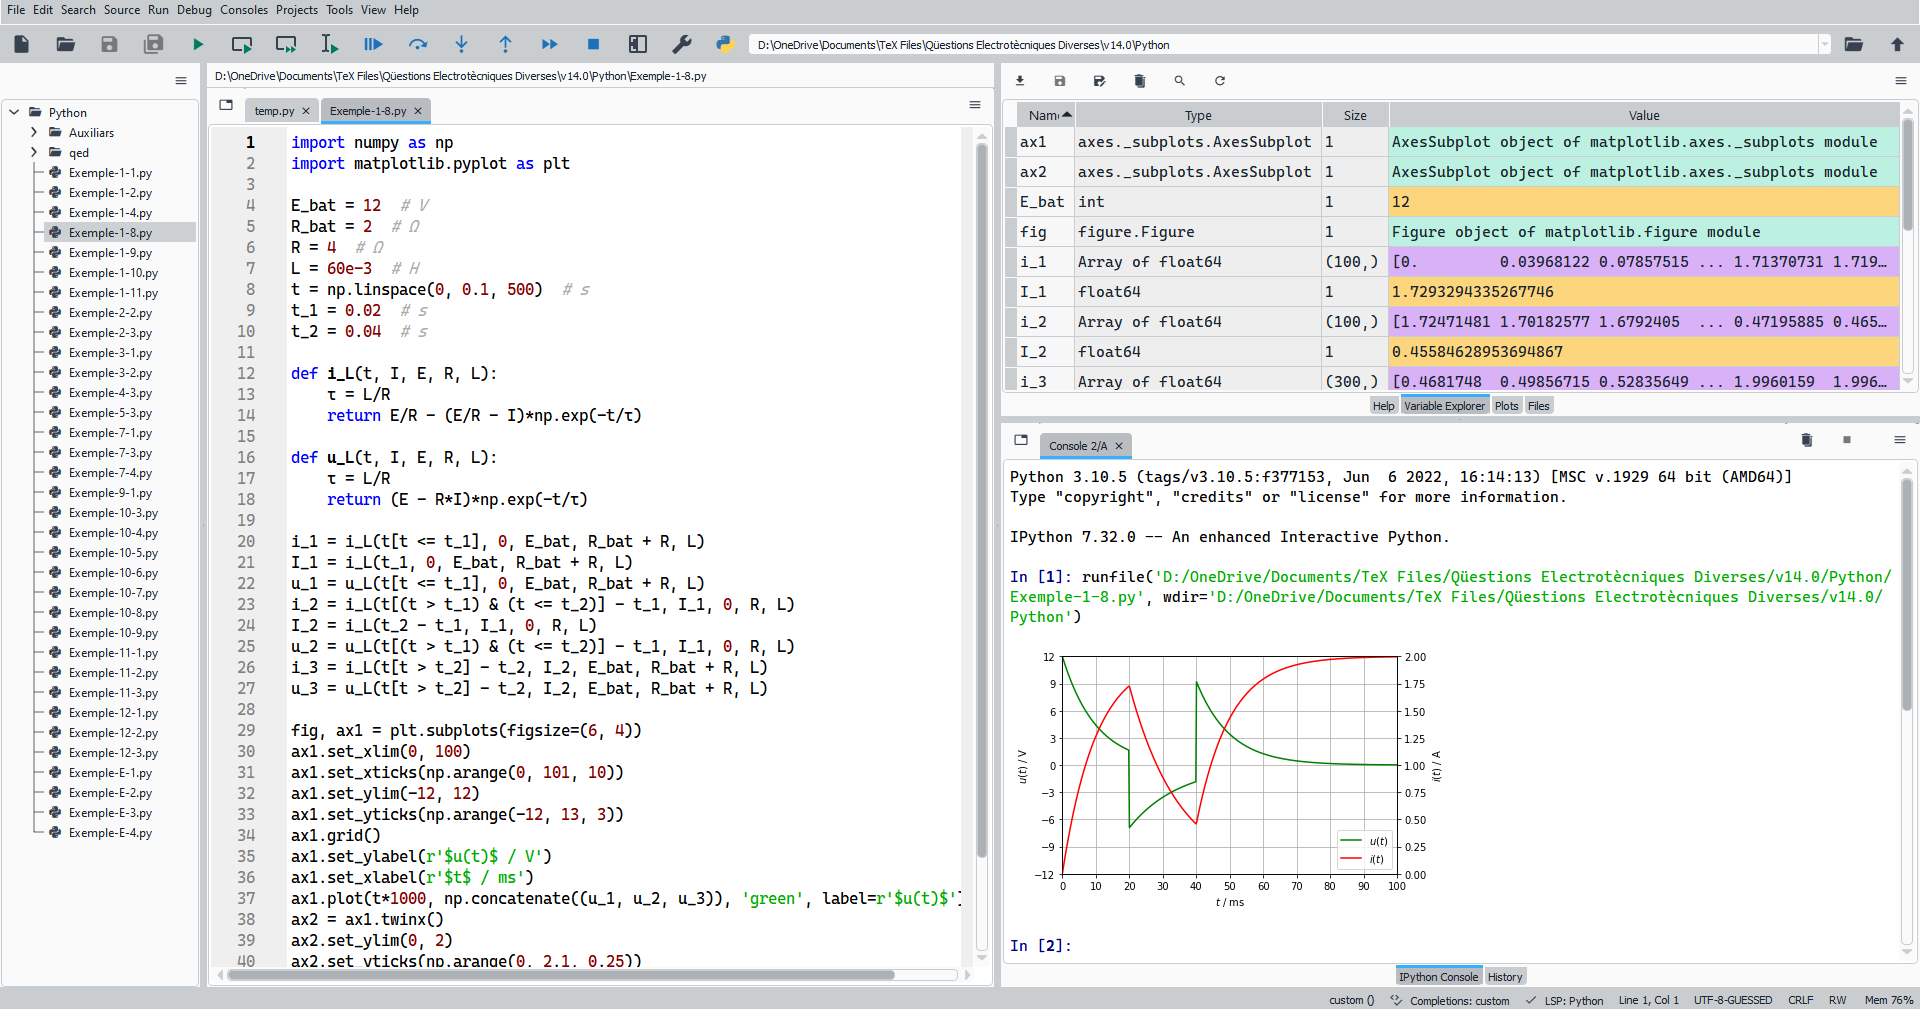
\includegraphics[width=\textwidth]{Cap-PythonLleng-Spyder.png}
	\captionof{figure}{IDE Spyder}
	\label{pic:spyder}
\end{center}


	

\section{Llibreries científiques}

Abans hem dit que els llenguatges interpretats s'executen més lentament que els compilats. Aquesta característica sembla que aniria en contra de l'elecció de Python com a llenguatge científic i tècnic, ja que en els algoritmes matemàtics de càlcul és crucial la velocitat per obtenir resultats en un temps raonable, sobretot quan el nombre de dades implicades és elevat.

La resolució d'aquesta  contradicció ve de la mà d'una sèrie de llibreries científiques que s'han anat desenvolupant durant anys i que avui dia estan plenament establertes. Aquestes llibreries tenen una sintaxi totalment compatible amb el llenguatge Python, però internament fan servir llibreries compilades, generalment en C o Fortran. D'aquesta manera s'aconsegueix la facilitat d'ús del llenguatge Python combinada amb la rapidesa d'execució dels llenguatges compilats.

En els apartats següents es descriuen breument  les llibreries científiques més útils i conegudes.

\subsection{NumPy}\index{NumPy}

NumPy  (\textit{Numerical Python}) és la llibreria numèrica bàsica; moltes altres la  fan servir com a base i punt de partida. El llibre de la referència \cite{VAN} en fa un tractament molt extens i detallat; també la tracten els llibres de les referències \cite{JOH} i \cite{HIL}.

El  web principal per obtenir informació d'aquesta llibreria és \href{https://numpy.org/}{numpy.org}.

La principal característica de NumPy és la manipulació eficient de variables dimensionades: vectors (una dimensió), matrius (dues dimensions), i variables de dimensió superior ($n$-dimensionals). Totes les operacions matricials s'efectuen de forma ràpida: suma, diferència, transposició, producte matricial, etc.

L'altra gran aportació de NumPy són les anomenades funcions universals (\funsfbs{ufunc}), les quals cobreixen tot l'espectre de les funcions matemàtiques usuals: aritmètiques, complexes, logarítmiques, trigonomètriques, hiperbòliques, etc. Aquestes funcions actuen sobre tots els elements d'una variable dimensionada, sense necessitat de programar un bucle per accedir a cada element de la variable d'un en un. 

El següent exemple s'executa en una sessió d'IPython utilitzant la funció màgica \funsfbs{\%timeit}; aquesta funció executa diverses vegades les instruccions que té a continuació i dona estadístiques del temps emprat. Per veure la diferència del temps d'execució entre el mòdul matemàtic \funsfbs{math} de Python  i NumPy, creem primer un vector amb 10 milions de valors i després calculem el sinus d'aquests valors; primer fem servir el mètode tradicional --- creant un bucle i calculant el sinus de cada valor un a un, amb la funció \funsfbs{sin} del mòdul \funsfbs{math} de Python ---, i en acabat utilitzem la funció universal \funsfbs{sin} de NumPy --- que no requereix cap bucle.

\begin{lstlisting}
In[1]: import math

In[2]: import numpy as np

In[3]: valors = np.linspace(0, 6.28, 10_000_000)   # Vector amb 10 milions de valors

In[4]: %timeit for x in valors: math.sin(x)  # Execució mitjançant un bucle
2.08 s ± 267 ms per loop (mean ± std. dev. of 7 runs, 1 loop each)

In[5]: %timeit np.sin(valors)  # Execució mitjançant una funció universal
94.8 ms ± 1.32 ms per loop (mean ± std. dev. of 7 runs, 10 loops each)

In[6]: 2.08/0.0948
Out[6]: 21.940928270042196
\end{lstlisting}

Com es pot veure, l'execució de NumPy és unes 22 vegades més ràpida que la del mòdul \funsfbs{math} de Python. Els valors concrets variaran d'una execució a la següent i dependran també de l'ordinador on s'executin aquestes instruccions, però queda clar que hi ha un guany significatiu de temps quan s'utilitzen les funcions universals de NumPy.


\subsection{SciPy}\index{SciPy}

SciPy (\textit{Scientific Python}) és la llibreria científica per exceŀlència, ja que proporciona algoritmes  matemàtics en moltes àrees del càlcul numèric. És compatible amb NumPy. Els llibres de les referències \cite{JOH} i \cite{HIL} en fan un bon tractament.

El  web principal per obtenir informació d'aquesta llibreria és \href{https://scipy.org/}{scipy.org}

Els principals camps  que cobreix SciPy són els següents:
\begin{itemize}
	\item \textbf{Funcions especials}. Funcions de Bessel, de Ricatti-Bessel, d'Struve,  d'Airy, de Fresnel, de Legendre, de Mathieu, de Kelvin, eŀlíptiques, hipergeomètriques, gamma, beta, d'error,  i moltes d'altres.
	\item \textbf{Integració}. Integració de funcions d'una o múltiples variables; integració de funcions a partir d'una mostra de punts (mètodes dels trapezis, de Simpson i de Romberg); resolució de sistemes d'equacions diferencials ordinàries amb valors inicials; resolució de sistemes d'equacions diferencials ordinàries amb condicions de contorn.
	\item \textbf{Optimització}. Minimització local de funcions d'una o múltiples variables; minimització global de funcions; resolució de problemes de mínims quadrats --- lineals i no lineals --- i ajust de corbes; càlcul d'arrels de funcions d'una o múltiples variables;  programació lineal.
	\item \textbf{Interpolació}. Interpolació polinòmica o per splines de funcions d'una o múltiples variables.
	\item \textbf{Transformada de Fourier}. Transformada ràpida de Fourier d'una o múltiples variables; transformada discreta del sinus i del cosinus; transformada ràpida de Hankel.
	\item \textbf{Processament de senyals}. Convolució, B-splies, filtrat, sistemes lineals de temps continu i discret, ones i anàlisi espectral.
	\item \textbf{Àlgebra lineal}. Sistemes d'equacions lineal, inversió de matrius i càlcul de determinats; valors i vectors propis; descomposició de matrius (LU, QR, etc.).
	\item \textbf{Estadística}. Distribucions de probabilitat contínues i discretes; valors i proves estadístiques; generació de variables aleatòries.
\end{itemize}


\subsection{SymPy}\index{SymPy}

SymPy (\textit{Symbolic Python}) és una llibreria de matemàtica simbòlica; és el que acostuma a anomenar-se un \textit{computer algebra system} (CAS). Proporciona resolucions simbòliques exactes a diversos problemes matemàtics. Addicionalment, pot transformar funcions simbòliques en numèriques, les quals poden usar-se amb SciPy. Els llibres de les referències \cite{JOH} i \cite{HIL} en fan un bon tractament.

El  web principal per obtenir informació d'aquesta llibreria és
\href{https://www.sympy.org/en/index.html}{www.sympy.org}

Els principals camps que cobreix SymPy són els següents:
\begin{itemize}
	\item \textbf{Funcions bàsiques}. Manipulació algebraica, expansió, simplificació i substitució; funcions matemàtiques: logarítmiques, trigonomètriques, hiperbòliques, gamma, zeta, esfèriques,  i d'altres.
	\item \textbf{Polinomis}. Divisió, factorització, 	 bases de Gröbner i descomposició en fraccions parcials.
	\item \textbf{Càlcul}. Diferenciació, integració, límits i sèries de Taylor.
	\item \textbf{Resolució d'equacions}. Algebraiques, polinòmiques i diferencials.
	\item \textbf{Combinatòria}. Combinacions, permutacions, particions i subconjunts.
	\item \textbf{Matemàtica discreta}. Sumatoris, productes, nombres primers i factorització.
	\item \textbf{Matrius}. Sistemes d'equacions, inversió, determinats, i valors i vectors propis.
	\item \textbf{Geometria}. Punts, rectes, polígons, cercles, intersecció, tangència i similitud.
	\item \textbf{Física}. Unitats, mecànica i òptica.
	\item \textbf{Estadística}. Funcions de probabilitat, probabilitats, i valors esperats  i variància.
\end{itemize}


\subsection{Matplotlib}\index{matplotlib}

Matplotlib és la llibreria més usada pel que fa a la representació gràfica de dades. Els llibres de les referències \cite{JOH}, \cite{HIL} i \cite{VAN} en fan un bon tractament.

El  web principal per obtenir informació d'aquesta llibreria és \href{https://matplotlib.org/}{matplotlib.org}

Matplotlib pot representar tota mena de gràfics en dues dimensions, i gràfics  tridimensionals de forma més limitada. Alguns dels tipus de gràfics que es poden obtenir són:
\begin{itemize}
	\item Funcions matemàtiques.
	\item Punts (\textit{scatter plot}).
	\item Barres.
	\item Histogrames.
	\item Caixes (\textit{boxplot}).
	\item Barres d'error.
	\item Pastís.
	\item Contorn.
	\item Polars.
	\item Logarítmics.
\end{itemize}

Tots els paràmetres dels gràfics són ajustables per part de l'usuari: gruix i color de línies i marcadors; font, mida i posició  del text;  títols i escales; posició i text de les marques dels eixos; i altres detalls.

Els gràfics generats per matplotlib poden exportar-se a diversos formats gràfics, tant de mapa de bits com vectorials: PNG, JPG, TIF, PDF, SVG, PS, i altres.



\subsection{Pandas}\index{pandas}

Pandas és una llibreria dedicada a la manipulació de dades.  El llibre de la referència \cite{VAN} en fa un tractament molt extens i detallat; també la tracten els llibres de les referències \cite{JOH}, \cite{HIL} i \cite{ZUM}.


El  web principal per obtenir informació d'aquesta llibreria és \href{https://pandas.pydata.org/}{pandas.pydata.org}

Les variables d'una dimensió (vectors) es tracten amb l'estructura \funsfbs{Series}, i les de dues dimensions (matrius) amb l'estructura \funsfbs{DataFrame}. L'estructura \funsfbs{DataFrame} es pot manipular d'una manera similar a com ho faríem amb un full d'Excel, de fet, pandas pot intercanviar dades amb fitxers Excel de manera senzilla.

